\section{Afstellen van de parameters}

Na de beslissingen die gemaakt werden in de eerdere secties, blijven er drie parameters over die de compressiefactor en -fout van de uitvoer bepalen: de relatieve doelfout tijdens de ST-HOSVD (RDS), de bits-parameter voor de quantisatie van de kerntensor (BPK) en de bits-parameter voor de quantisatie van de factormatrices (BPF). Het is echter niet triviaal om deze drie optimaal te kiezen om bijvoorbeeld de compressiefactor te maximaliseren met bij een bepaalde compressiefout. In deze sectie zullen we proberen een algoritme te ontwerpen dat in beperkte rekentijd goede parameterwaarden kan bepalen.\\

Helaas duurt de compressie en decompressie van grote datasets te lang om met een groot aantal parameterwaarden te experimenteren, dus we zullen ons in onze analyse beperken tot twee kleinere gevallen: Cuprite en Indian Pines.

\subsection{Niet-adaptieve selectie}

Om een idee te krijgen van de optimale parameterwaarden voor een bepaalde relatieve fout, zullen we eerst een groot aantal experimenten uitvoeren met vari\"erende waarden. Hierbij gebruiken we de volgende domeinen:

\begin{itemize}
\item $RDS \in \{0.005, 0.075, 0.01, \dots, 0.05\}$
\item $BPK \in \{16, 15, 14, \dots, 1\}$
\item $BPF \in \{16, 15, 14, \dots, 1\}$
\end{itemize}

We kunnen aannemen dat (bijna altijd) het verhogen van de RDS, verlagen van de BPK of verlagen van de BPF de uiteindelijke compressiefout zal vergroten. Daarnaast zijn we vooral ge\"interesseerd in relatieve doelfouten kleiner dan 0.05. Bijgevolg zullen we, eens dat er een experiment een fout voorbij deze grens gaf, geen experimenten meer proberen met grotere (of gelijke) RDS en lagere (of gelijke) BPK en BPF, want deze geven sowieso een grotere fout. Op deze manier kunnen we de parameterruimte sneller doorzoeken.

\begin{figure}[H]
  \centering
  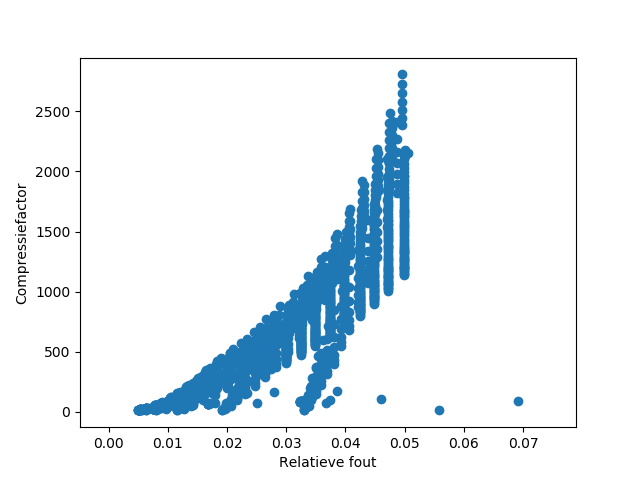
\includegraphics[scale=0.7]{images/all_sweep_points_cuprite.png}
  \caption{Resultaten voor vari\"erende parameters voor Cuprite. Elk punt stelt \'e\'en experiment voor, met een unieke combinatie van parameterwaarden.}
  \label{fig:all_sweep_points_cuprite}
\end{figure}

In figuur \ref{fig:all_sweep_points_cuprite} zien we de volledige verzameling uitgevoerde experimenten op \'e\'en grafiek (voor Cuprite). De meeste punten zijn echter niet interessant. Stel namelijk, elk experiment $E_i$ geeft een relatieve fout $RF_i$ en compressiefactor $CF_i$. Als men dan twee experimenten $E_i$ en $E_j$ beschouwt, met $RF_i < RF_j$ en $CF_i > CF_j$, dan is het resultaat van $E_i$ op beide vlakken beter en is $E_j$ zeker een suboptimaal resultaat. Na het wegfilteren van dergelijke suboptimale punten bekomen we de curve uit figuur \ref{fig:filtered_sweep_points_cuprite}. Vanaf nu zullen we dit de steekproefoptima noemen, aangezien deze nog steeds gelimiteerd zijn door de eerder gekozen domeinen voor de parameterwaarden. Vooral voor grote fouten begint deze beperking merkbaar te worden en wordt de curve minder continu.

\begin{figure}[H]
  \centering
  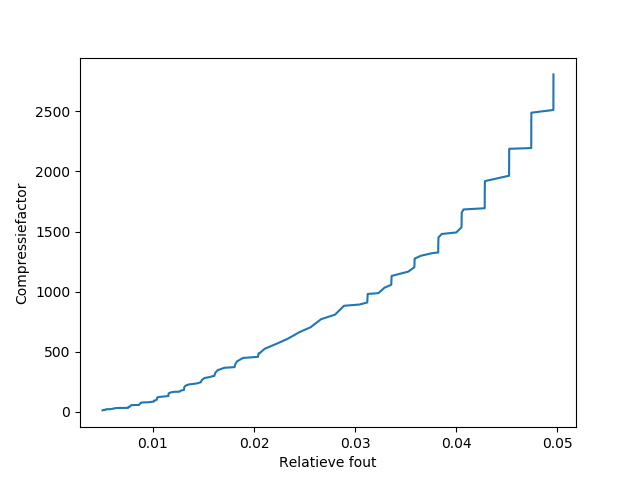
\includegraphics[scale=0.7]{images/filtered_sweep_points_cuprite.png}
  \caption{Resultaten voor vari\"erende parameters voor Cuprite, zonder suboptimale punten.}
  \label{fig:filtered_sweep_points_cuprite}
\end{figure}

In figuren \ref{fig:filtered_sweep_points_RDS}, \ref{fig:filtered_sweep_points_BPK} en \ref{fig:filtered_sweep_points_BPF} zien we welke parameterwaarden corresponderen met deze steekproefoptima. We voerden ook hetzelfde proces uit op Indian Pines. Voor elke parameter leggen we nu een selectiefunctie vast op basis van deze experimentele resultaten. Het kiezen van deze functies kan geavanceerder en is zeker een piste voor verder onderzoek.

\begin{itemize}
\item $RDS = max(0.001, 0.962601*\text{kwaliteit} - 0.000414)$, simpelweg op basis van lineaire regressie. De resultaten voor Cuprite en Indian Pines liggen hier vrij dichtbij elkaar.
\item $BPK = max(10, round(-445.117*\text{kwaliteit} + 16.795))$. Deze functie werd bepaald aan de hand van lineaire regressie op de eerste waarden van Cuprite, gevolgd door een harde ondergrens van 10. Dit is weliswaar te groot voor Indian Pines, maar zoals we eerder zagen kan de fout erg snel escaleren wanneer het aantal quantizatiebits te laag gekozen wordt, dus we zullen gaan voor eerder conservatieve waarden.
\newpage

\begin{figure}[H]
  \centering
  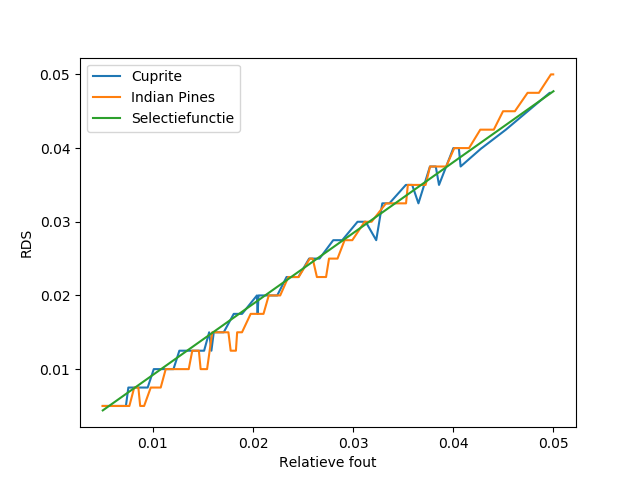
\includegraphics[scale=0.7]{images/filtered_sweep_points_RDS.png}
  \caption{RDS-waarden van steekproefoptima en de RDS-selectiefunctie.}
  \label{fig:filtered_sweep_points_RDS}
\end{figure}

\begin{figure}[H]
  \centering
  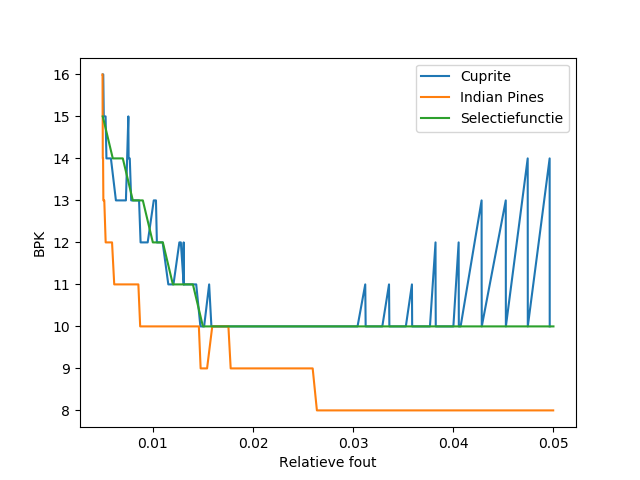
\includegraphics[scale=0.7]{images/filtered_sweep_points_BPK.png}
  \caption{BPK-waarden van steekproefoptima en de BPK-selectiefunctie. De grote sprongen bij de laatste waarden van Cuprite worden veroorzaakt door de beperkte selectie van RDS-waarden gedurende de experimenten.}
  \label{fig:filtered_sweep_points_BPK}
\end{figure}

\newpage

\begin{figure}[H]
  \centering
  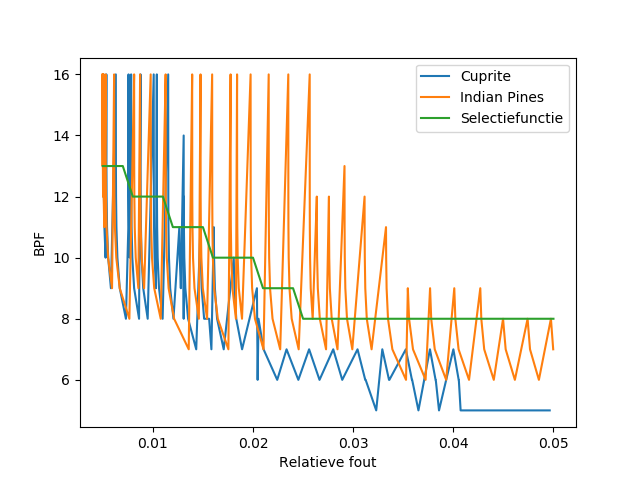
\includegraphics[scale=0.7]{images/filtered_sweep_points_BPF.png}
  \caption{BPF-waarden van steekproefoptima en de BPF-selectiefunctie.}
  \label{fig:filtered_sweep_points_BPF}
\end{figure}

\item $BPF = max(8, round(-228.571*quality + 14.143))$. We zien in de experimentele resultaten dat de exacte steekproefoptima sterk vari\"eren, dus we kozen ervoor om vooral naar het midden van de functies te kijken (we zullen zien dat dit geen plotselinge grote fouten geeft in onze eindresultaten, zie figuren \ref{fig:parameter_functions_results_Cuprite} en \ref{fig:parameter_functions_results_Indian_Pines}). Deze selectiefunctie werd gekozen op analoge wijze als de BPK-functie, maar deze keer net beperkt door resultaten van Indian Pines.
\end{itemize}

Met deze selectiefuncties hebben we compressies uitgevoerd waarbij de RDS, BPK en BPF automatisch bepaald werden op basis van \'e\'en enkele parameter, de kwaliteit. Als waarden voor de kwaliteitsparameter gebruikten we 0.005, 0.006, \dots, 0.05. De resultaten hiervan kan men vinden in figuren \ref{fig:parameter_functions_results_Cuprite} en \ref{fig:parameter_functions_results_Indian_Pines}. Voor kleine fouten lijken onze functies goed te werken, maar naarmate de fout stijgt verliezen we een deel van onze compressiefactor vanwege suboptimale parameterkeuzes.

\newpage
\begin{figure}[H]
  \centering
  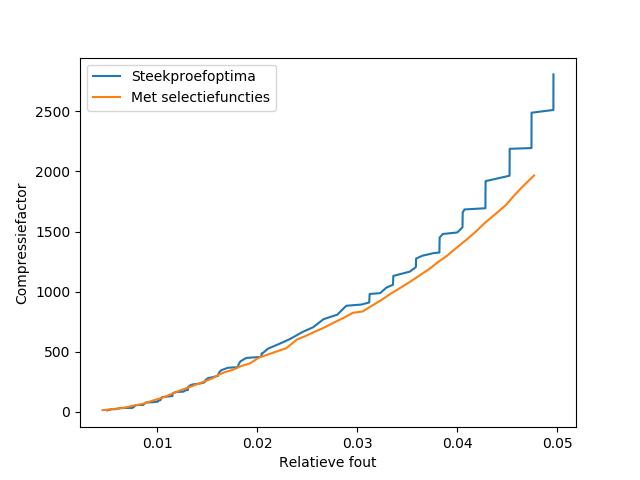
\includegraphics[scale=0.7]{images/parameter_functions_results_Cuprite.png}
  \caption{Resultaten van compressie met selectiefuncties voor Cuprite.}
  \label{fig:parameter_functions_results_Cuprite}
\end{figure}

\begin{figure}[H]
  \centering
  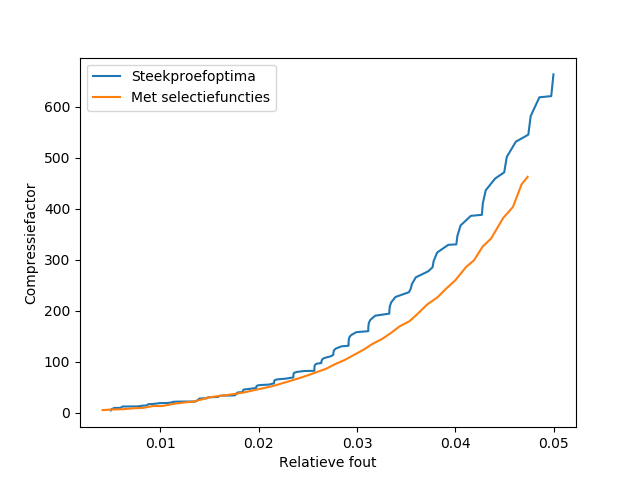
\includegraphics[scale=0.7]{images/parameter_functions_results_Indian_Pines.png}
  \caption{Resultaten van compressie met selectiefuncties voor Indian Pines.}
  \label{fig:parameter_functions_results_Indian_Pines}
\end{figure}

\newpage
\subsection{Adaptieve selectie}

Als we meer rekentijd mogen investeren, kunnen we echter betere parameters kiezen door gedurende de compressie simpelweg verschillende waarden uit te proberen en het beste resultaat te kiezen. Bij adaptieve selectie zullen we dit in beperkte mate proberen te doen.\\

Concreet maken we van de compressie een iteratief algoritme, waarbij we starten met dezelfde parameters als bij niet-adaptieve selectie. We zagen eerder dat de RDS-functie vrij onafhankelijk is van de dataset, waardoor we deze parameterwaarde niet meer zullen aanpassen. In elke iteratie testen we de uiteindelijke compressiefout en -factor zowel als men de BPK-waarde of de BPF-waarde met \'e\'en zou verlagen. Het algoritme kiest dan op basis van het huidige resultaat en de alternatieve resultaten welke parameter verlaagd wordt voor de volgende stap (de exacte beslissingsprocedure laten we hier buiten beschouwing). Als geen van beide verlaagd kan worden zonder dat de compressiefout de kwaliteitsparameter overschrijdt, stopt het algoritme.\\

Bij de implementatie werd weliswaar rekening gehouden met enkele optimisaties:
\begin{itemize}
\item Aangezien de RDS-waarde vast ligt, moet de ST-HOSVD en orthogonaliteitscompressie slechts \'e\'en keer uitgevoerd worden, zelfs met vari\"erende BPK en BPF.
\item Bij het berekenen van de alternatieve compressies, moet telkens maar de helft van de quantisatie- en encoderingsfasen uitgevoerd worden: alleen de kerntensor moet herberekend worden voor verlaagde BPK, alleen de factormatrices voor verlaagde BPF.
\item Elke iteratie moet slechts \'e\'en nieuw alternatief berekend worden, want het alternatief van de parameter die niet verlaagd werd kan hergebruikt worden. Het kost wel extra geheugen om deze compressies bij te houden.
\end{itemize}

In figuren \ref{fig:parameter_functions_results_including_adaptive_Cuprite} en \ref{fig:parameter_functions_results_including_adaptive_Indian_Pines} vindt men de experimentele resultaten van adaptieve parameterselectie. Men ziet dat men met deze techniek grote vooruitgang kan boeken op vlak van compressiefout en -factor. Door het beperkte domein van de RDS-waarden in de initi\"ele steekproef (waarmee we de optimale parameterwaarden probeerden te analyseren) verslaat adaptieve selectie zelfs de steekproefoptima.\\

In figuren \ref{fig:adaptive_timings_Cuprite} en \ref{fig:adaptive_timings_Indian_Pines} zien we echter dat adaptieve parameterselectie een significante kost heeft op vlak van compressietijd. Verder wordt er ook meer geheugen gebruikt voor het bijhouden van alternatieve compressies. Om deze redenen zullen we deze techniek in het algemeen proberen te gebruiken, tenzij de uitvoeringstijd naar ons oordeel onacceptabel is.

\newpage
\begin{figure}[H]
  \centering
  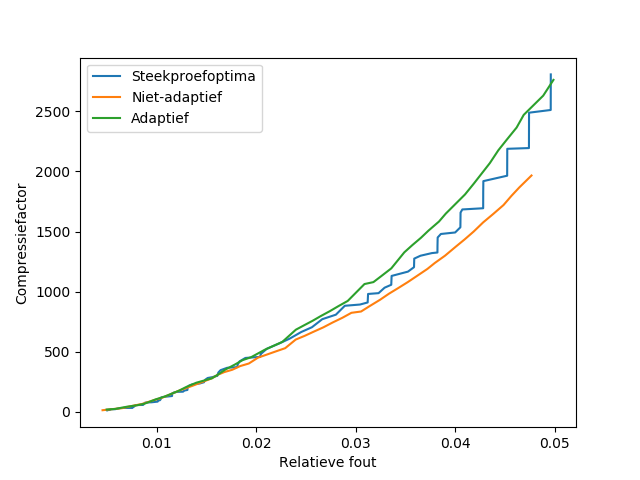
\includegraphics[scale=0.7]{images/parameter_functions_results_including_adaptive_Cuprite.png}
  \caption{Resultaten van compressie met adaptieve parameterselectie voor Cuprite.}
  \label{fig:parameter_functions_results_including_adaptive_Cuprite}
\end{figure}

\begin{figure}[H]
  \centering
  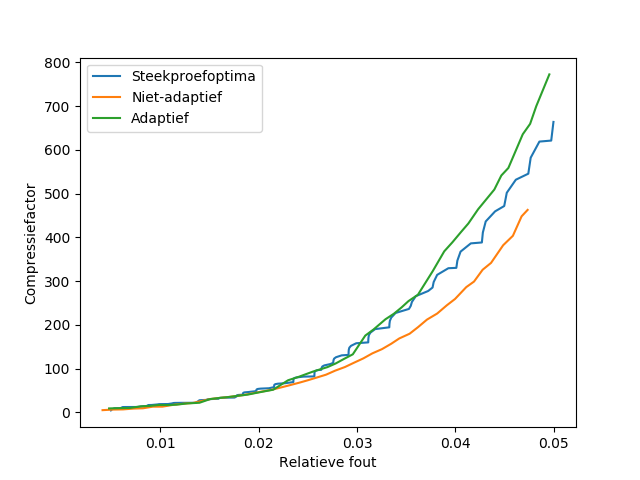
\includegraphics[scale=0.7]{images/parameter_functions_results_including_adaptive_Indian_Pines.png}
  \caption{Resultaten van compressie met adaptieve parameterselectie voor Indian Pines.}
  \label{fig:parameter_functions_results_including_adaptive_Indian_Pines}
\end{figure}

\newpage
\begin{figure}[H]
  \centering
  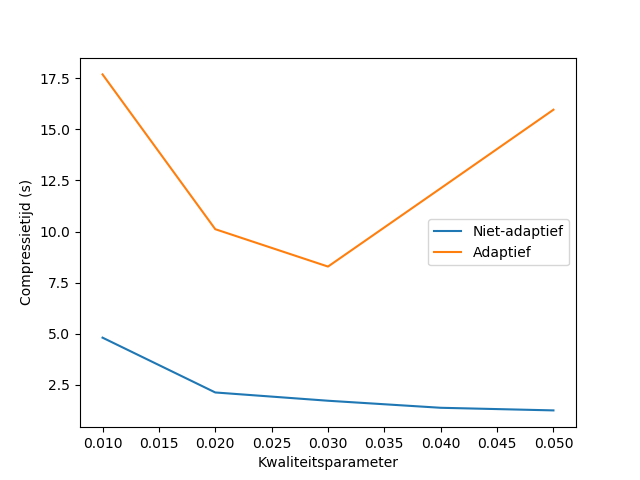
\includegraphics[scale=0.7]{images/adaptive_timings_Cuprite.png}
  \caption{Gemiddelde compressietijden voor verschillende kwaliteitsparameters voor Cuprite (10 experimenten).}
  \label{fig:adaptive_timings_Cuprite}
\end{figure}

\begin{figure}[H]
  \centering
  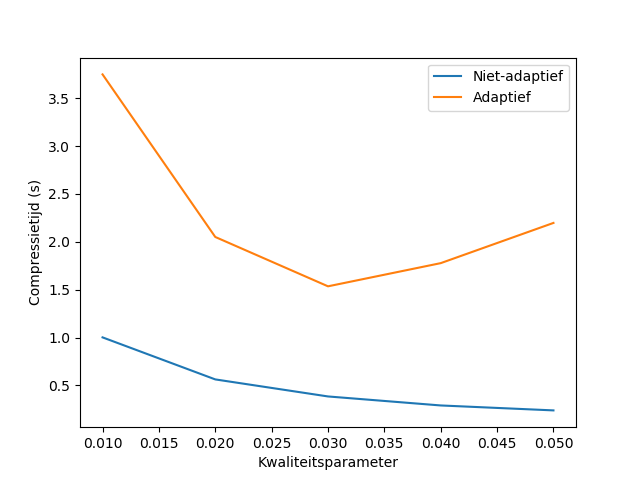
\includegraphics[scale=0.7]{images/adaptive_timings_Indian_Pines.png}
  \caption{Gemiddelde compressietijden voor verschillende kwaliteitsparameters voor Indian Pines (10 experimenten).}
  \label{fig:adaptive_timings_Indian_Pines}
\end{figure}
